\documentclass[10pt]{article}

\usepackage[accepted]{rlc}
% If accepted, instead use the following line for the camera-ready submission:
%\usepackage[accepted]{rlc}
% To de-anonymize and remove mentions to RLC (for example, for posting to preprint servers), instead use the following:
% \usepackage[preprint]{rlc}

\usepackage{array}
\usepackage{amsmath}
\usepackage{amsthm}
\usepackage{amsbsy}
\usepackage{amssymb}
\newtheorem{definition}{Definition}
\usepackage{graphicx}
\usepackage{mathtools}
\usepackage{nicefrac}
\usepackage{bm}
\usepackage{enumitem}
\usepackage{mpemath}
\usepackage{tcolorbox}
\usepackage[capitalize,noabbrev]{cleveref}
\usepackage{theoremref}
\usepackage{thmtools}
\usepackage{thm-restate}
\usepackage{algorithm}
\usepackage{algpseudocode}
\usepackage{tikz}
\usepackage{subcaption}

\bibliographystyle{abbrvnat}
\usepackage[framemethod=default]{mdframed}

\renewcommand{\cite}{\citep}

%\mathtoolsset{showonlyrefs}     % Only number equations that are referenced (optional)
\usepackage{bbm}

\renewcommand{\algorithmicrequire}{\textbf{Input:}}
\renewcommand{\algorithmicensure}{\textbf{Output:}}
\newcommand{\cvar}{\text{CVaR}}
\newcommand{\cvaralpha}{\text{CVaR}_\alpha}
\newcommand{\var}{\text{VaR}}
\newcommand{\varalpha}{\text{VaR}_\alpha}


\theoremstyle{plain}
\newtheorem{theorem}{Theorem}
\newtheorem{lemma}{Lemma} 
\newtheorem{proposition}{Proposition}
\newtheorem{assumption}{Assumption}
\theoremstyle{remark}
\newtheorem{example}{Example}

% \newcommand{\mm}[1]{\textcolor{magenta}{[#1]}}
% \newcommand{\db}[1]{\textcolor{blue}{[DB: #1]}}
% \newcommand{\gersi}[1]{\textcolor{red}{[#1]}}
% \newcommand{\s}[1]{\mathcal{#1}}

\DeclareMathOperator{\ext}{ext}

% \setlength{\parskip}{3mm plus 1mm minus 1mm}
% \setlength{\parindent}{0pt}

\title{Survey on Risk-Averse Reinforcement Learning}
\author{Gersi Doko \\
        Gersi.Doko@unh.edu \\}


\begin{document}

\maketitle

\section{Introduction}

Reinforcement learning (RL) is a powerful framework for developing agents that can learn to make decisions in complex, uncertain environments.
The core goal of RL is to tractably compute an optimal policy for acting in such an environment. A key challenge in RL is 
that the environment is often stochastic, and the agent may have only partial observability. 
Choosing an objective function that accurately captures the desired behavior of the agent is a difficult task.

We would hope the objective that an RL agent aims to optimize would consider the "risk" of the actions it takes.
One first needs to consider how to quantify risk into a numerical value. A value that encapsulates the uncertainty of the outcome of an action,
so that an agent can distinguish between actions that are risky and those that are safe.

There is a vast field of research that focuses on developing risk measures.
The goal of a risk measure is to quantify the uncertainty of a random variable, often while being interpretable and computationally tractable.
The intersections of risk and reinforcement learning is the topic of this review, where we will explore the field of risk-averse reinforcement learning.

\section{Risk and Reward}

\begin{definition}[Risk Measure]
        \label{def:risk}
        A Risk Measure is a mapping from a random variable to a real number. Quantifying the uncertainty of an outcome.
        Given a metric space ($\Omega$, $\mathcal{F}$, $P$), a risk measure is a function $\psi: \mathcal{X} \to \Real$. Satisfying
        \begin{enumerate}
                \item Monotonicity: $X \leq Y \implies \psi(X) \leq \psi(Y)$
                \item Translation Invariance: $\psi(X + c) = \psi(X) + c \quad \forall c \in \Real$
        \end{enumerate}
\end{definition}

\begin{definition}[Variance]
        \label{def:variance}
        The variance of a random variable $X$ is defined as 
        $$\text{Var}(X) = \mathbb{E}[(X - \mathbb{E}[X])^2].$$
\end{definition}

\begin{definition}[Expectation]
        \label{def:expectation}
        A common risk measure is the expectation of a random variable. Given a random variable $X: \Omega \to \Real$, the expectation of $X$ is defined as
        $$\mathbb{E}[X] = \sum_{\omega \in \Omega} X(\omega) P(\omega).$$
\end{definition}

\begin{definition}[Value at Risk (Var)]
        The Value-at-Risk (VaR) of a random variable $X$ at risk-level $\alpha$ is defined as
        $$\varalpha(X) = \inf \left\{ t \in \Real \mid P(X \leq t) \geq \alpha \right\}.$$
\end{definition}

\begin{definition}[Conditional Value-at-Risk (CVaR)]
        \label{def:cvar}
        The Conditional Value-at-Risk (CVaR) of a random variable $X$ at risk-level $\alpha$ is defined as
        $$\cvaralpha(X) = \min_{t \in \Real} \left\{ t + \frac{1}{1 - \alpha} \mathbb{E}[(X - t)_+] \right\}.$$
\end{definition}


\begin{figure}[ht!]
        \begin{subfigure}[t]{0.5\textwidth}
                \centering
                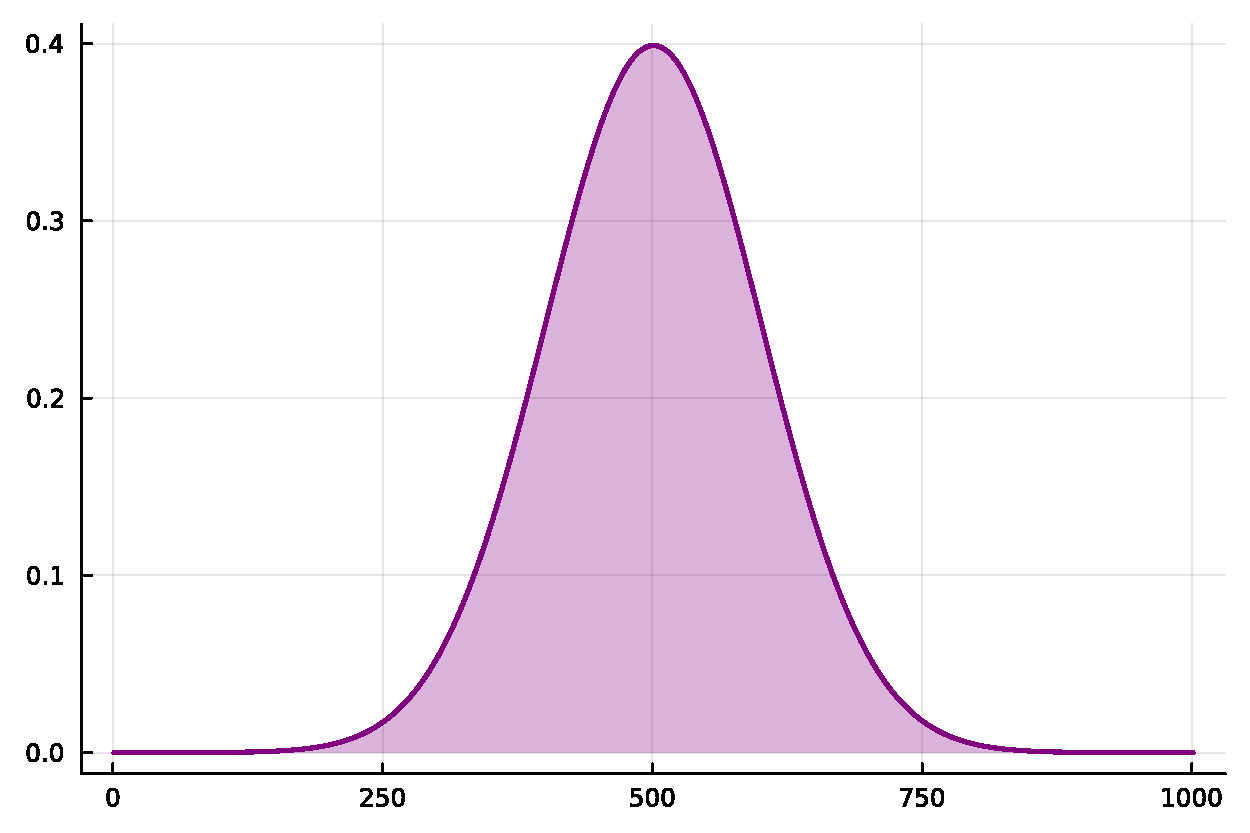
\includegraphics[width=0.7\linewidth]{julia_figures/normal.pdf}
                \caption{$\mathcal{N}(0,1)$}
                \label{fig:normal}
        \end{subfigure}
        \begin{subfigure}[t]{0.5\textwidth}
                \centering
                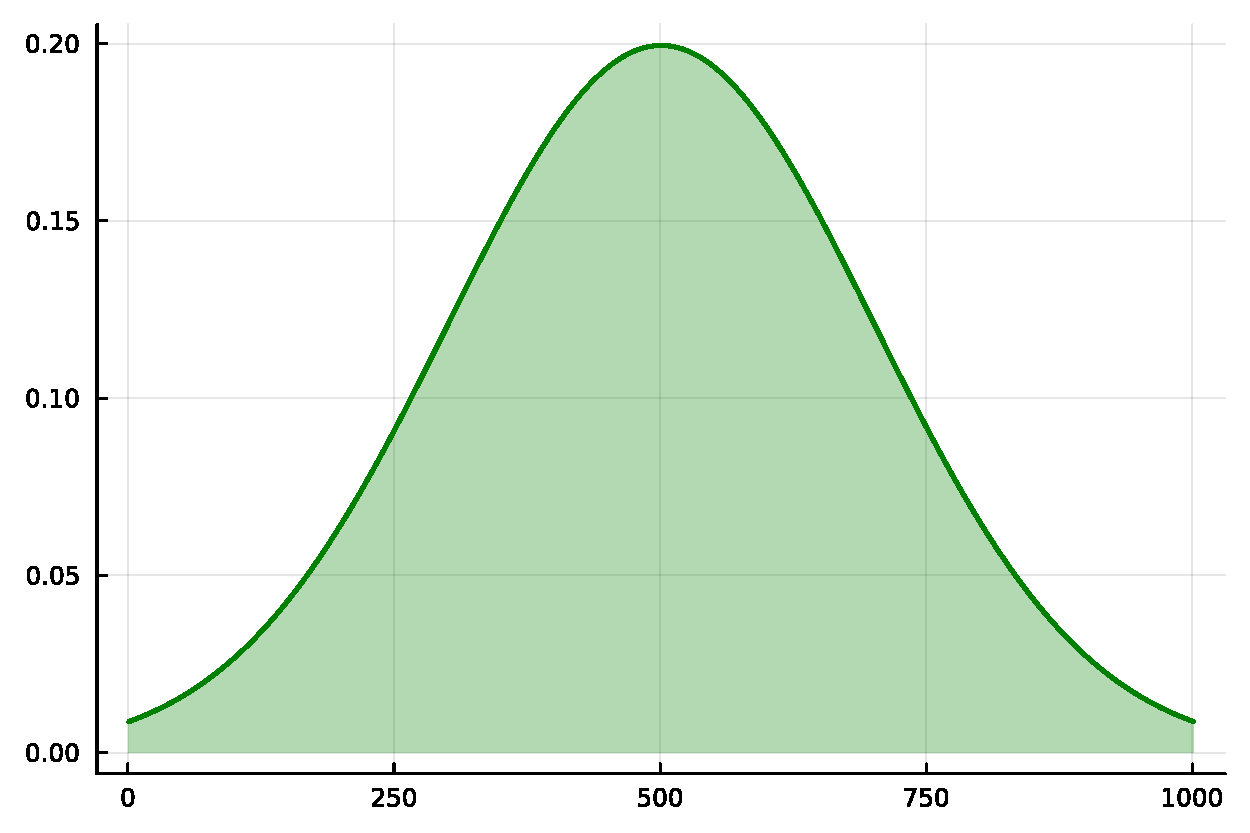
\includegraphics[width=0.7\linewidth]{julia_figures/normal_wide.pdf}
                \caption{$\mathcal{N}(0,2)$}
                \label{fig:normal_wide}
        \end{subfigure}
        \begin{subfigure}[t]{1.0\textwidth}
                \centering
                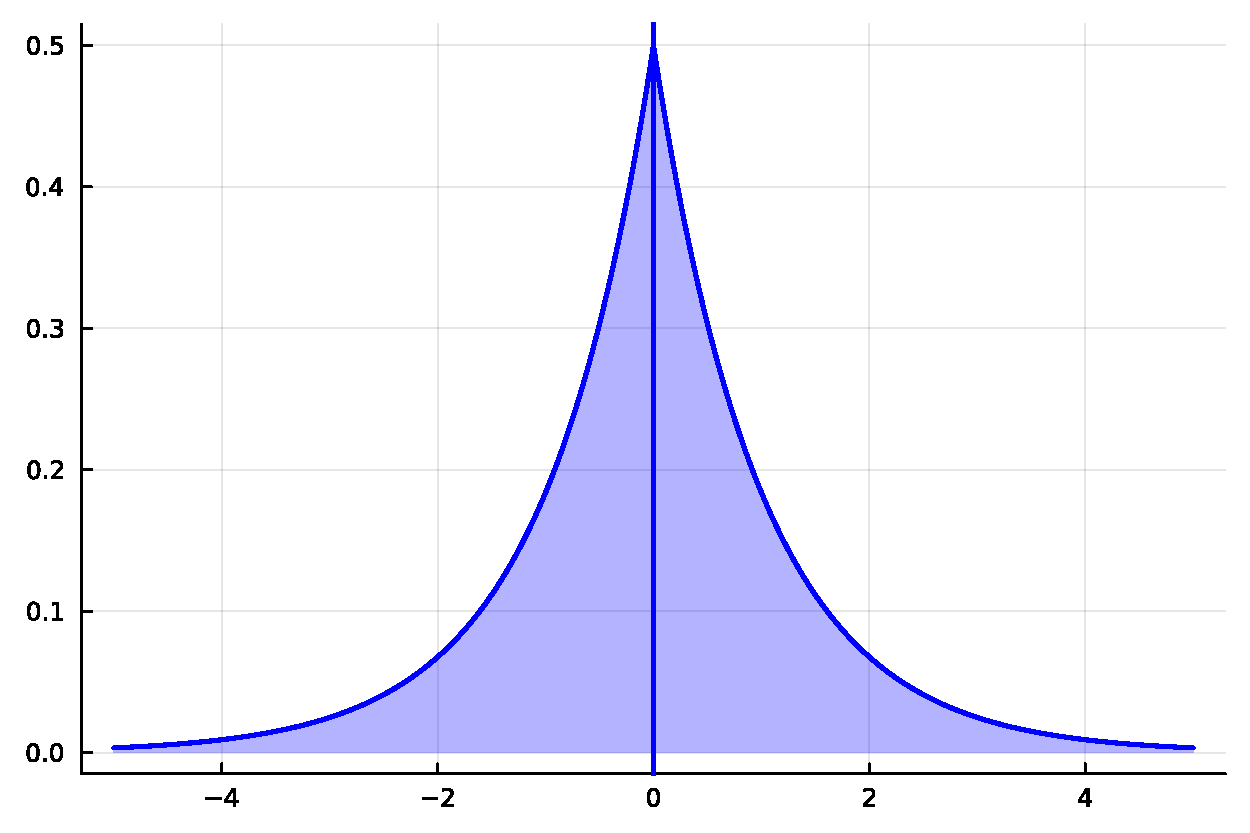
\includegraphics[width=0.4\linewidth]{julia_figures/laplace.pdf}

                \caption{$\mathcal{L}(0,1)$}
                \label{fig:laplace}
        \end{subfigure}
        \caption{Probability Density Functions of Various Distributions. All with a shared mean of 0.}
        \label{fig:pdfs}
\end{figure}

\section{Vanilla Reinforcement Learning}

\begin{definition}[Finite Horizon Expected Return]
        Given a policy $\pi : \mathcal{S} \to \Delta^\mathcal{A}$ the expected finite horizon discounted return $\rho(\pi)$ can be defined as
        $$\rho(\pi) = \mathbb{E}_{\pi, \mathcal{P}} \left[ \sum_{t=0}^{T} \gamma^t r(s_t, \pi(s_t)) \right].$$
        Where $s_0 \sim p_0$ and $s_{t+1} \sim \mathcal{P}(s_t, \pi(s_t))$, $\gamma$ is the discount factor, and $T$ is the time horizon.
\end{definition}

\begin{definition}[Objective of Reinforcement Learning]
        \label{def:rl_obj}
        The objective of reinforcement learning (RL) is as follows
        $$\max_{\pi \in \Pi} \rho(\pi).$$
        Where $\Pi = \left\{ \pi \in \mathcal{S} \to \Delta^\mathcal{A}  \right\}$.
        In practice, one is most concerned with the optimal policy $\pi^* = \argmax_{\pi \in \Pi} \rho(\pi)$.
\end{definition}

\section{Risk-Averse Reinforcement Learning}

\section{Methods}

\end{document}
